\chapter{A Correlated Green Kubo Counterexample and the Limits of Spectral Tests}\label{ch:counterexample}

\section{Why an explicit counterexample is necessary}
A necessary and sufficient algebraic condition becomes a useful physical classification only if the conditions on both sides are compatible with admissible response dynamics. Otherwise the nonrigid branch might be a formal possibility excluded by stability, positivity, or stationarity. This chapter constructs a minimal correlated stochastic process that retains the two component rotational form and positive dissipation while leaving the anchored circle.

The model is not proposed as a microscopic representation of FHP collisions. Its purpose is sharper: it is a witness against the claim that symmetry plus positive dissipation alone protect CRTC.

\section{Stationary two component Ornstein Uhlenbeck process}
Let $X(t)\in\mathbb{R}^2$ obey
\begin{equation}
 \dd X=-K(d)X\,\dd t+B(d)\,\dd W,
 \label{eq:ou_sde}
\end{equation}
where $W$ is a two component Wiener process and
\begin{equation}
 K(d)=a(d)I+b(d)J,
 \qquad
 J=\begin{pmatrix}0&-1\\1&0\end{pmatrix}.
 \label{eq:ou_k}
\end{equation}
Choose
\begin{equation}
 a(d)=a_0+\epsilon d^2,
 \qquad
 b(d)=cd,
 \qquad
 a_0>0,
 \quad\epsilon>0.
 \label{eq:ou_functions}
\end{equation}
The eigenvalues of $K$ are
\begin{equation}
 q_\pm=a(d)\pm i b(d).
 \label{eq:ou_eigenvalues}
\end{equation}
Their real parts are positive for every real $d$, so the process is linearly stable.

Reflection maps $d\mapsto-d$ and changes the sign of $b$ while leaving $a$ unchanged. The drift therefore has the same parity structure allowed by the shear commutant calculation in \cref{ch:rigidity}.

\section{Stationary covariance and positive dissipation}
Fix an isotropic stationary covariance
\begin{equation}
 C=A I,
 \qquad A>0.
 \label{eq:ou_cov}
\end{equation}
The Lyapunov equation for stationarity is
\begin{equation}
 K C+C K^{T}=B B^{T}.
 \label{eq:ou_lyapunov}
\end{equation}
Since $J^T=-J$,
\begin{equation}
 K C+C K^{T}=2Aa(d)I.
 \label{eq:ou_noise}
\end{equation}
This matrix is positive definite because $A>0$ and $a(d)>0$. One may therefore choose a real noise amplitude $B$ whose covariance is \cref{eq:ou_noise}. The symmetric part of the drift is $a(d)I>0$, so the dissipative sector is positive.

The reactive coordinate $bJ$ does not contribute to the symmetric quadratic dissipation. This is the same algebraic separation between dissipative and odd components that makes the model useful as a counterexample.

\section{Exact Green Kubo integral}
For a stationary Ornstein Uhlenbeck process,
\begin{equation}
 \langle X(t)X(0)^T\rangle=\e^{-K t}C.
 \label{eq:ou_correlation}
\end{equation}
Because the eigenvalues of $K$ have positive real part,
\begin{equation}
 R(d)=\int_0^\infty\e^{-K t}C\,\dd t
 =K^{-1}C.
 \label{eq:ou_gk}
\end{equation}
The integral is exact and already includes temporal correlations of the stationary process. After division by the positive scalar $A$, the normalized complex response is
\begin{equation}
 Z(d)=\frac{1}{a(d)+i b(d)}.
 \label{eq:ou_z}
\end{equation}
The response therefore lies in precisely the class covered by \cref{eq:defect_ab}, but its dissipative inverse coordinate drifts with $d$.

Substitution gives
\begin{equation}
 \boxed{
 \Delta(d)=
 -\frac{\epsilon d^2}
 {a_0\left[(a_0+\epsilon d^2)^2+c^2d^2\right]}}
 \label{eq:ou_defect}
\end{equation}
which is strictly negative for $d\ne0$. The model is stable, stationary, rotationally covariant in the two component sector, reflection covariant, and positively dissipative, yet it does not preserve the anchored circle.

\begin{figure}[htbp]
\centering
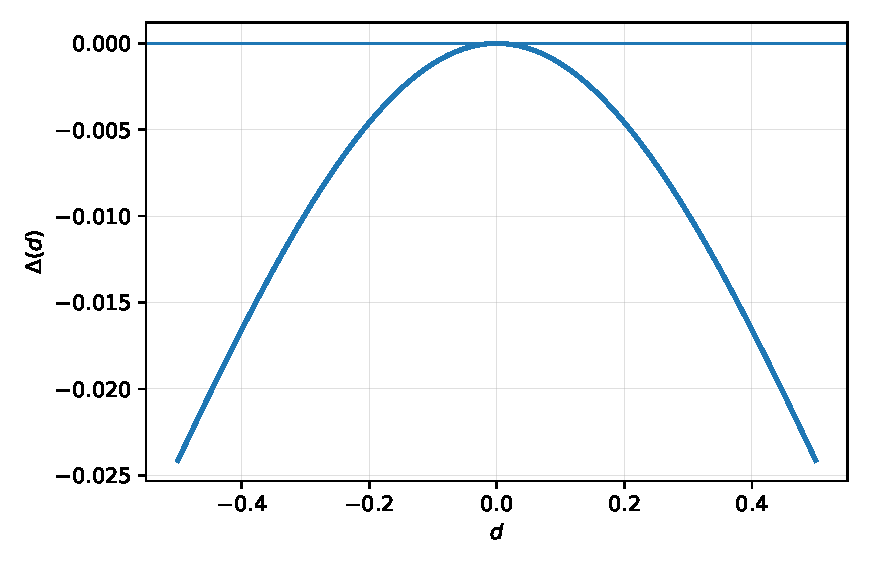
\includegraphics[width=.76\textwidth]{ou_counterexample_defect.pdf}
\caption{Exact counterexample defect for $a_0=3/2$, $\epsilon=2/5$, and $c=9/10$ on the finite rational test domain. The curve is generated from \cref{eq:ou_defect}; it is not fitted data.}
\label{fig:ou_defect}
\end{figure}

\section{Finite exact counterexample certificate}
The executable test uses
\begin{equation}
 a_0=\frac32,
 \qquad
 \epsilon=\frac25,
 \qquad
 c=\frac9{10},
 \label{eq:ou_test_params}
\end{equation}
and evaluates
\begin{equation}
 d=\frac{i}{1000},
 \qquad
 i=-500,\ldots,500.
 \label{eq:ou_test_grid}
\end{equation}
All arithmetic is rational. The domain contains \CRTCCounterGridPoints{} points. The test proves $a(d)>0$ at every point, obtains zero defect at $d=0$, and obtains a strictly negative defect at each of the remaining \CRTCCounterOffCircle{} points.

The finite sweep is a regression check for the explicit family, while \cref{eq:ou_defect} is the continuum proof. In particular, the sign of the defect is known analytically for every real nonzero $d$ when the stated positive parameters are used.

\section{The rigid correlated class is nonempty}
Set $\epsilon=0$ while keeping $a_0>0$ and $b(d)=cd$. The same stochastic construction has
\begin{equation}
 K(d)=a_0I+cdJ,
 \label{eq:ou_rigid_k}
\end{equation}
positive symmetric dissipation, a stationary isotropic covariance, and exact Green Kubo response
\begin{equation}
 Z(d)=\frac1{a_0+icd}.
 \label{eq:ou_rigid_z}
\end{equation}
By \cref{eq:defect_ab}, its defect vanishes identically. Thus the admissible class contains both rigid and nonrigid members. The distinction is not correlation versus no correlation; it is whether the dissipative part of the measured inverse response is flat in chirality.

\section{What can be decided from a spectrum}
In an identified two dimensional shear block of the form $aI+bJ$, the eigenvalues are
\begin{equation}
 q_\pm=a\pm ib.
 \label{eq:shear_spectrum}
\end{equation}
If the response normalization or residue is known so that these eigenvalues are indeed the inverse response coordinates, the circle criterion is immediate: compare their common real part with the achiral value. No time domain simulation is required.

This statement must not be expanded to an arbitrary microscopic spectrum. A Green Kubo coefficient has the schematic resolvent form
\begin{equation}
 \mathcal{R}=\langle g,L^{-1}h\rangle
 \label{eq:resolvent_matrix_element}
\end{equation}
on the nonconserved subspace. Eigenvalues of $L$ matter, but so do eigenvectors, spectral projectors, and the overlaps of the observable and source with those modes.

The CRTC package includes an exact two dimensional witness. Let
\begin{equation}
 L_1=\begin{pmatrix}1&0\\0&2\end{pmatrix},
 \qquad
 S=\begin{pmatrix}1&1\\0&1\end{pmatrix},
 \qquad
 L_2=S L_1S^{-1}.
 \label{eq:same_spectrum_matrices}
\end{equation}
The matrices are similar and therefore have exactly the same spectrum. With fixed $g=(1,0)$ and $h=(0,1)^T$, however,
\begin{equation}
 gL_1^{-1}h\ne gL_2^{-1}h.
 \label{eq:different_overlap}
\end{equation}
The bare unordered full spectrum is therefore insufficient to determine a general response matrix element.

\section{Meaning for collision operators}
The distinction suggests a practical decision tree. If a microscopic analysis isolates the exact shear invariant subspace, identifies its effective generator, and fixes the response residue, then the complex pair can decide CRTC membership algebraically. If additional slow variables mix with shear, or if only the full list of eigenvalues is known, one must project or eliminate the additional variables and compute the actual scalar complex response before applying the theorem.

This is particularly relevant beyond molecular chaos. Correlations can generate a frequency dependent self energy or memory kernel. A two component form may survive symmetry reduction, but its coefficients can depend on frequency, size, and chirality. The classifier remains valid at each fixed prescription:
\begin{equation}
 \RePart\!\left[\frac1{Z_{L,\omega}(p)}\right]
 =\RePart\!\left[\frac1{Z_{L,\omega}(p_0)}\right]
 \label{eq:regulated_classifier}
\end{equation}
if and only if the regulated response lies on its anchored circle.

\section{Chapter conclusion}
The counterexample closes the structural classification at the level that symmetry and positivity can address. There exists a correlated positive dissipation rigid class and a correlated positive dissipation nonrigid class. Consequently $C_6$, reflection parity, stationarity, and positivity do not determine the outcome. An identified reduced shear spectrum can decide membership, while a bare full spectrum generally cannot. The remaining task is therefore model specific: determine the actual correlated inverse shear response of the chiral FHP automaton or prove an identity that constrains it.
